\documentclass[10pt,a4paper]{article}
\usepackage[utf8]{inputenc}
\usepackage[italian]{babel}
\usepackage{amsmath}
\usepackage{amsfonts}
\usepackage{amssymb}
\usepackage{graphicx}
\usepackage[left=2cm,right=2cm,top=2cm,bottom=2cm]{geometry}
\newcommand{\rem}[1]{[\emph{#1}]}

\author{Gruppo BN \\ Federico Belliardo, Marco Costa, Lisa Bedini}
\title{Esperienza sull'effetto fotoelettrico}
\begin{document}

\maketitle
\section{Scopo dell'esperienza}
Obiettivo dell'esperienza � la verifica dell'effetto fotoelettrico, e di stimare la grandezza del fattore $h/e$, dove $h$ � la costante di Planck e $e$ la carica dell'elettrone\\
%forse mettere la fomrletta E = h\nu?
\section{Materiale occorrente}
\begin{itemize}
\item Lampada a LED;
\item Tubo fotomoltiplicatore Philips XP2412 B;
\item Filtri interferenziali (Balzers e Newport);
\item Scatola nera
\item Generatore di tensione continua;
\item Multimetro digitale;
\item Picoamperometro digitale;
\end{itemize}
\section{Descrizione esperimento}

%TODO
Si � montato il circuito in figura \ref{circuito}. Nella scatola nera erano fissati il fotomoltiplicatore e la lampada a LED che serviva da sorgente luminosa. Durante l'esperienza, si sono montati i filtri nell'apposito supporto, avendo cura che fossero ortogonali al piano di appoggio della scatola e quindi al fascio luminoso.

Si � montato il circuito in figura \ref{fig:circuito}. Nella scatola nera erano fissati il fotomoltiplicatore e la lampada a LED che serviva da sorgente luminosa. Durante l'esperienza, si sono montati i filtri nell'apposito supporto, avendo cura che fossero ortogonali al piano di appoggio della scatola e quindi al fascio luminoso.


Per ogni filtro si � misurata la corrente in funzione del potenziale applicato ai capi del fotomoltiplicatore. Per un certo potenziale $V_0$ la corrente di elettroni (estratti per effetto fotoelettrico) che arriva all'amperometro si arresta. Questo ci consente di stimarne la massima energia cinetica degli elettroni come $eV_0$, da confrontare con l'energia dei fotoni incidenti $E_{\gamma}=h\nu$.
\begin{figure}[!htb]
  \centering
  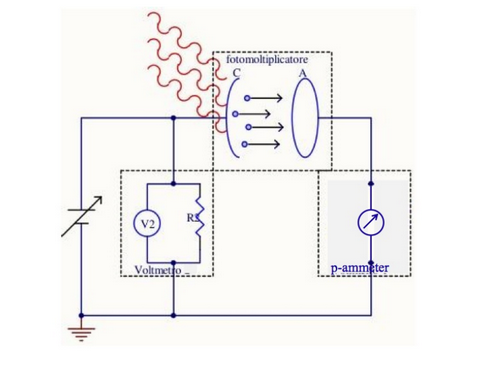
\includegraphics[scale=.5]{circuito.png}
\caption{Schema circuito dell'esperimento e di acquisizione dati.\label{circuito}}
\end{figure}


\section{Misure}

Per ogni filtro si sono prese venti misure di tensione ai capi del tubo fotomoltiplicatore e della relativa corrente.
Si � partiti da $V\simeq 0$ V e si � variato il potenziale fino a che la corrente non raggiungeva un valore asintotico. Si sono preferite prendere misure nella regione asintotica e intorno al punto in cui il grafico curvava significativamente: in questo modo ci � stato pi� facile estrarre i parametri nei fit dei punti successivi della relazione.
La tensione di frenamento � stata misurata tramite multimetro digitale. La corrente circolante nel circuito � stata misurata tramite picoamperometro.
La lettura della corrente veniva fatta dopo un tempo sufficientemente lungo da fare in modo che il valore riportato dallo strumento si fosse stabilizzato.
Come errori si sono presi gli errori strumentali riportati sui manuali dello strumento.%(0.5\% + 1 digit per il voltmetro e 0.4\% + 1 digit e 0.2\% + 1 digit per il picoamperometro, rispettivamente sulle scale dei 20 nA e dei 200 nA
Per stimare le lunghezze d'onda dei filtri, e quindi della frequenza effettiva dei fotoni incidenti, si � usata la tabella fornita (si veda la tabella \ref{tab:filtri}).
L'incertezza associata ad ogni lunghezza d'onda riportata � stata presa come la semidispersione della banda passante.
 \begin{table}[!ht]
\begin{center}
\begin{tabular}{|c|c|c|}
\hline 
Colore & $\lambda$ (nm) & Tipo \\ 
\hline 
Arancione & $602\pm$ & Balzers\\ 
\hline 
Giallo & $577\pm$ & Newport\\ 
\hline 
Verde & $546\pm$ & Balzers\\ 
\hline 
Verde-azzurro & $499\pm $ & Newport\\ 
\hline 
Azzurro & $ 449\pm$ & Balzers \\ 
\hline
Blu & $405\pm$ & Newport\\ 
\hline
\end{tabular} 
\caption{Caratteristiche dei filtri utilizzati \label{tab:filtri}}
\end{center}
\end{table}

Di seguito sono riportate le tabelle dei dati raccolti per ogni filtro.\\
\section{Elaborazione dati: stima potenziale di azzeramento $V_0$}
Per trovare la relazione fra frequenza dei fotoni incidenti e il relativo potenziale di azzeramento � necessario stimare dai dati quest'ultimo. Per fare ci� abbiamo usato due metodi.
\subsection{Metodo A}
Per ogni filtro si stima la corrente di emissione dall' anodo $I_A$. In prima approssimazione, si suppone che questa non dipenda significativamente dal potenziale di frenamento applicato. Pertanto si assume che la fotocorrente catodica sia $I_{C}$ sia $I-I_A$. 
Dati gli andamenti della corrente, si esegue un fit con la funzione modello $\sqrt(I_C)=aV +b$.
Una volta estratti i parametri, si trova il potenziale di azzeramento $V_0$ ponendo $I_{C}=0\rightarrow V_0=-b/a$.
Per stimare la corrente di emissione dell'anodo, si sino presi i dati in regime asintotico e si � eseguito un fit con costante.
I risultati dei fit sono riportati nelle tabelle  \ref{}

\subsection{Metodo B}
Per ogni filtro si � stimato il relativo potenziale di azzeramento $V_0$ corrispondente alla tensione per cui la corrente fotocatodica risulta compatibile con 0 entro l'incertezza $\delta I$.
 Per fare ci� si � eseguito un fit per ogni set di misure con la funzione modello
\begin{equation}
I(V)=\bar{I}(e^{a(\bar{V}-V})}-1)
\end{equation}
Si osservi che con questa definizione $\bar(I)$ rappresenta il modulo della  corrente asintotica misurata.
Per ricavare $V_0$ basta risolvere l'equazione
\begin{equation}
I(V_0)=-\bar{I}+\delta(I)\Rightarrow V_0=\bar{V}+\frac{1}{a}\ln\frac{\bar{I}}{\delta I}
\end{equation} 
Come incertezza $\delta I$ si � preso l'errore sul parametro estratto da ogni fit.
SICuro????
\section{Relazione frequenza-$V_0$}
Una volta ottenuti i potenziali di azzeramento per le varie frequenze, si esegue un fit secondo la funzione modello $V=a\nu + b$.
Secondo il modello, $a = h/e$ e b rappresenta il lavoro di estrazione necessario per portare l'elettrone fuori dalla banda di conduzione.
\section{Conclusioni}


\end{document}


